% example tikz figure

\documentclass{standalone}
\usepackage{amsmath}
\usepackage{amsfonts}
\usepackage{tikz}
\usetikzlibrary{arrows,shapes,positioning,shadows,trees}


\begin{document}

\begin{tikzpicture}
    \node (a) at (0,0) {
        \begin{tikzpicture}
            % draw elipse x^2/4 + y^2 = 1, and rotate that counterclockwise by 45 degrees
            % \draw [-] plot [smooth, tension=] coordinates {(2,0) (0,1) (-2,0) (0,-1) (2,0)};
            % \draw [-] plot [smooth, tension=1] coordinates {(2,0) (0,2) (-2,1) (-1.5,-2) (1,-2) (2,-1) (2,0)};
            \draw (0,0) [rotate=45] ellipse (2cm and 1cm);
            \node[below right] at (1, -1) {$G$};


            \node[fill,circle,inner sep=1pt,label=below right:$z_0$] at (-1,-0.5) {};

            \node[fill,circle,inner sep=1pt,label=above:$z_n$] at (1,0.5) {};
            \node[fill,circle,inner sep=1pt,label=left:$z_n^{'}$] at (0.5,-0.5) {};

            \draw[-] (0.5,-0.5) -- (1,0.5);

            \node[fill,circle,inner sep=1pt,label=right:$S$] at (1.414 / 2 + 0.5, - 1.414 / 2 + 0.6) {};

            % draw circle around node above, with radius 1. dotted line
            \draw[dotted] (1.414 / 2 + 0.5, - 1.414 / 2 + 0.6) circle (1.5);
        \end{tikzpicture}
    };


    \node (b) at (8,0) {
        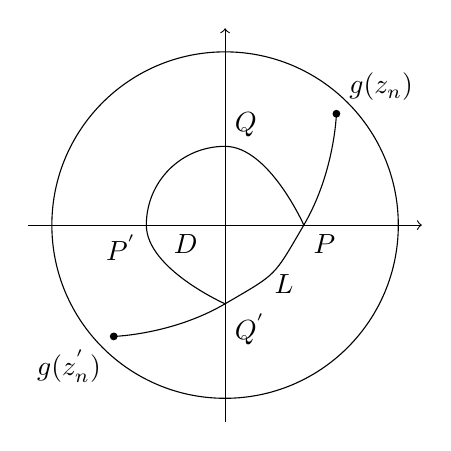
\begin{tikzpicture}
            % fill under circle (0,0) radius 1
            \draw (0,0) circle (2.2);

            % axis
            \draw[->] (-2.5,0) -- (2.5,0);
            \draw[->] (0,-2.5) -- (0,2.5);

            \node[fill,circle,inner sep=1pt,label=above right:$g(z_n)$] at (1.414, 1.414) {};
            \node[fill,circle,inner sep=1pt,label=below left:$g(z_n^{'})$] at (-1.414, -1.414) {};

            \draw [-] plot [smooth, tension=1] coordinates {(1,0) (0,1) (-1,0) (0,-1)};
            \draw [-] plot [smooth, tension=1] coordinates {(1.414, 1.414) (1,0) (0,-1) (-1.414, -1.414)};

            \node[below right] at (1,0) {$P$};
            \node[below left] at (-1,0) {$P^{'}$};
            \node[above right] at (0,1) {$Q$};
            \node[below right] at (0,-1) {$Q^{'}$};


            \node[below] at (-0.5,0) {$D$};

            \node[below] at (0.75,-0.5) {$L$};

        \end{tikzpicture}
    };

    \draw[->] (a) -- (b);
    \node[above] at (3.5,0) {$g$};
\end{tikzpicture}
\end{document}